\chapter{陈省身微分几何讲义}\index{陈省身微分几何讲义}
\section{流形的基本概念}\index{流形的基本概念}
\begin{thm}
\begin{enumerate}[label=(\arabic*),font=\upshape]
    \item 给定 $M,N$ 为两个 $n$维光滑流形且 $f$是从 $M$到 $N$的光滑映射.\cite{吴大任1979微分几何讲义}
    \item 在 $M$上一点 $p$处, $f$诱导的切映射 $f_*\colon T_p (M)\to T_{f(p)}(N)$是同构.
\end{enumerate}
则存在一点$p$在 $M$中的邻域 $U$, 使得 $V=f(U)$为 $f(p)$在 $N$中一邻域且 $f|_U\colon U\to V$是可微同胚.
\end{thm}
\begin{proof}
    由于 $f:M\to N$ 是光滑映射.故取 $p$在 $M$中局部坐标系 $(U_),\varphi)$和 点 $q=f(p)$在 $N$中局部坐标系 $(V_0,\psi)$,使得 $f(U_0)\subseteq V_0$,且
    \begin{eq*}
        \tilde{f}=\psi\circ f \circ \varphi^{-1}\colon \varphi (U_0)\to \psi (V_0) \subset \R^n.
    \end{eq*}
    是光滑映射.
    \begin{figure}[h]
        \begin{small}
            \begin{center}
                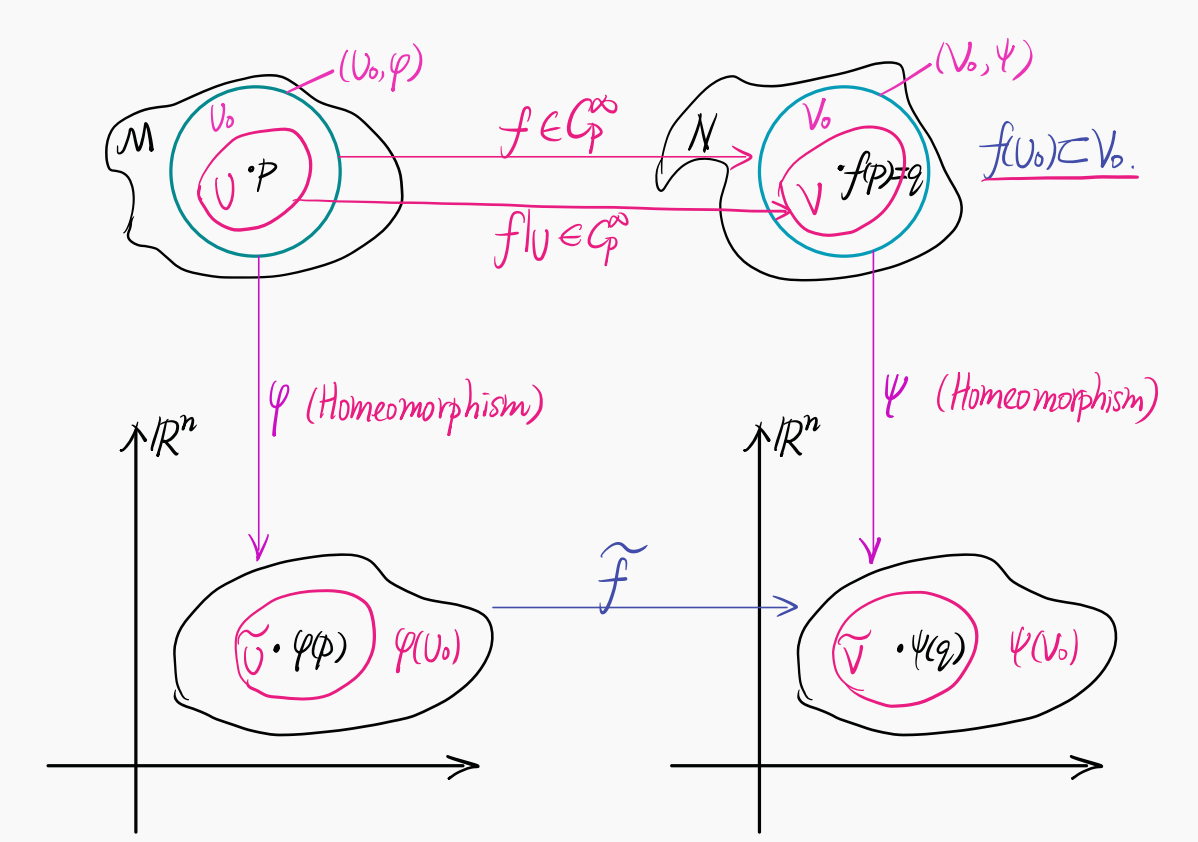
\includegraphics[width=0.6\textwidth]{figures/thm3.4.png}
            \end{center}
            \caption{图示}
            \label{fig:thm3.4proof}
        \end{small}
    \end{figure}
    
    故 $\tilde{f}=\psi\circ f\circ \varphi^{-1}$是光滑的. $\varphi(U_0)$与 $\psi(V_0)$均是 $\R^n$中的开集.在定理3.1中,令 $x_0=\varphi(p),f=\tilde{f}$,则若 $\det \left(\frac{\partial f^i}{\partial x^j}\right)\bigg|_{x_0}\neq 0$,则存在 $\varphi(p)$与$\psi(q)$在 $\varphi(U_0)$与 $\psi(V_0)$的邻域 $\widetilde{U}$与 $\widetilde{V}$,使得 $\tilde{f}|_{U_0}\colon \widetilde{U}\to\widetilde{V}$是可微同胚.
    令 $U=\varphi^{-1}(\widetilde{U}),V=\psi^{-1}(\widetilde{V})$,则 $U$与 $V$分别是$p$与 $q$在 $M$与 $N$中的邻域,且$f|_{U}=\psi^{-1}\circ \tilde{f}\circ \varphi\colon U\to V$是可微同胚.

    为何 $\tilde{f}$在 $\varphi(p)$的Jacobi行列式非零是显然的?
    由于
    \[
    \begin{aligned}
        & \left.\operatorname{det}\left(\frac{\partial f^i}{\partial x^j}\right)\right|_{x_0} \neq 0 . \Leftrightarrow f_*: T_{x_0} M\left(\simeq \mathbb{R}^n\right) \longrightarrow T_{f_{(x_0)}}\left(\mathbb{R}^n\right)\left(\simeq \mathbb{R}^n\right) \\
        & \left.\operatorname{det}\left(\frac{\partial \tilde{f}^i}{\partial x^j}\right)\right|_{\varphi(p)} \neq 0 \Leftarrow \tilde{f}_*: T_{\varphi(p)} M \left(\simeq \mathbb{R}^n\right) \longrightarrow T_{\tilde{f} \varphi(\rho)}\left(\mathbb{R}^n\right) (\simeq \mathbb{R}^n) 
        \end{aligned}\]
        故映射 $f$的 Jacobi矩阵 $\left(\frac{\partial f^i}{\partial x^j}\right)$恰是 $f_*$在自然基底下的矩阵.
\end{proof}
\subsection{小结}
\subsubsection*{余切空间}
\begin{itemize}
    \item 余切空间 $T^*_p =\F_p/\mathcal{H}_p=\{(\dd f)_p\}$,
    \item 自然基底 $\{(\dd u^i)_p,1\leqslant i\leqslant n\}$,
    \item 余切空间之间的光滑映射:
    \[F^*\colon T^*_q\to T^*_p\; \text{(设 $F\colon M\to N$是光滑映射且 $q=F(p)$.)}\]
    \begin{itemize}[label=\twicecircle]
        \item 作用方式 \quad $(\dd f)_p\mapsto \dd(f\circ F)$,
        \item 在两个自然基底下的矩阵表示: 
        
        设 $u^i$是 $p$附近的局部坐标表示, $v^\alpha$是 $q$附近的局部坐标表示,则映射 $F$在点$p$附近可用函数
        \begin{equation}
            \label{eq:valpha}
            v^\alpha=F^\alpha (u^1,\cdots,u^m),1\leqslant \alpha\leqslant n,
        \end{equation}
        表示.

        注解: \begin{eq*}
            v^\alpha &=(\psi(q))^\alpha=(\psi\circ F(p))^\alpha=(\psi\circ F\circ \varphi^{-1}(u^1,\cdots,u^m))^\alpha\\
            &\xlongequal[]{\text{令 $F^\alpha=\psi\circ F\circ \varphi^{-1}$}} F^\alpha (u^1,\cdots,u^m)
        \end{eq*}
        因此, $F^*$在自然基底 $\{\dd v^\alpha,1\leqslant\alpha\leqslant n\}$作用下结果为
        \begin{eq*}
                    F^* (\dd v^\alpha)=\dd (v^\alpha\circ F)=(\dd (F^\alpha(u^1,\cdots,u^m)))_p=\sum_{i=1}^{m}\left(\frac{\partial F^\alpha}{\partial u^i}\right)_p \cdot (\dd u^i).
        \end{eq*}
        从而 $F^* \{\dd v^\alpha\}=J\{\dd u^i\}$,其中 $J=\left(\frac{\partial F^\alpha}{\partial u^i}\right)_p$为 \eqref{eq:valpha}函数的Jacobi矩阵.
    \end{itemize}
    \item 余切向量的自然基底表示
    
    设 $\alpha=\dd f\in T_p^*$,则 $\alpha=\sum_{i=1}^{m}a_i \dd u^i, a_i=\frac{\partial f}{\partial u^i} \quad (\text{这里将复合映射仍记为$f$},  f=f\circ \varphi_U^{-1})$ (由定理 2.2)
    \item 坐标变换 (在不同坐标系$u^i$与$u^{*i}$下同一向量坐标变化)
    
    设另一局部坐标$u^{*i}$,则$\alpha$关于自然基底的表示式为$\alpha=\sum_{i=1}^{m}a_i^* \dd u^{*i}$,其中$a_i=\sum_{i=1}^{m}a_j^* \frac{\partial u^{*j}}{\partial u^i}$,且 $\frac{\partial u^{*j}}{\partial u^i}=\frac{\partial (\varphi_{U*}\circ \varphi_U^{-1})}{\partial u^i}$那么
    \begin{eq}
        \alpha &=(\dd u^1,\cdots,\dd u^m)\overrightarrow{\beta}, \overrightarrow{\beta}=(a_1,\cdots,a_m)^\prime \\ 
        &=(\dd u^{*1},\cdots,\dd u^{*m})\overrightarrow{\beta^*}, \overrightarrow{\beta}=(a_1^*,\cdots,a_m^*)^\prime
    \end{eq}
    又
    \begin{eq*}
        (\dd u^{*1},\cdots,\dd u^{*m})&=(\dd u^1,\cdots,\dd u^m)T\\
        &=(\dd u^1,\cdots,\dd u^m)(T\overrightarrow{\beta^*})
    \end{eq*}
即有$T\overrightarrow{\beta^*}=\overrightarrow{\beta}$.
由$T=\left(\frac{\partial u^{*j}}{\partial u^i}\right)\bigg|_{(ij)}$,故 $a_i=\sum_{i=1}^{m}a_j^* \cdot \left(\frac{\partial u^{*j}}{\partial u^i}\right)$.
\end{itemize}
\begin{remark}
    \begin{enumerate}[font=\upshape]
        \item $u^i (1\leqslant i\leqslant m)$称为点 $q\in U$ ($U$为$p$在$M$中的邻域)的局部坐标,即
        \begin{eq*}
            u^i=(\varphi_U(q))^i,\quad q\in U, 1\leqslant i\leqslant m
        \end{eq*}
        \item \Figure{width=.5\linewidth}{figures/11.png}{余切空间图示}{fig:cotangent space}
    \end{enumerate}
\end{remark}
\subsubsection*{切空间}
\begin{itemize}
    \item 切空间 $T_p=\{\langle [\gamma], (\dd f)_p\rangle, \gamma\in \Gamma_p\}$.
    \item 自然基底 $\{[\lambda_k],1\leqslant k\leqslant m\}=\left\{\left(\frac{\partial}{\partial u^k}\right)_p, 1\leqslant k\leqslant m\right\}$.
    \item 切空间之间的光滑映射 ($F^*$的共轭映射)(也称为相伴映射)
    \[F_*\colon T_p\to T_q,\]
    \begin{itemize}[label=\twicecircle]
        \item 作用方式: $\langle F_* X,\alpha\rangle=\langle X,F^* \alpha\rangle, X\in T_p,\alpha\in T_q^*$.
        \item 在两个自然基底下的矩阵表示
        
        切映射$F_*$在自然基底$\left\{\frac{\partial }{\partial u^i}\right\}$上的作用是
        \begin{eq}
            \langle F_*\left(\frac{\partial }{\partial u^i}\right),\dd v^\alpha\rangle &=\lan{\frac{\partial}{\partial u^i},F^*(\dd v^\alpha)}\\ 
            &=\sum_{i=1}^{m}\lan{\frac{\partial }{\partial u^i},\dd u^i}\cdot \left(\frac{\partial F^\alpha}{\partial u^i}\right)_p\\ 
            &=\lan{\sum_{i=1}^{m}\left(\frac{\partial F^\beta}{\partial u^i}\right)_p \frac{\partial }{\partial v^\beta},\dd v^\alpha}.
        \end{eq}
        即 $F_*\left(\frac{\partial }{\partial u^i}\right)=\sum_{\beta=1}^{m}\left(\frac{\partial F^\beta}{\partial u^i}\right)_p \frac{\partial }{\partial v^\beta}$.
    \end{itemize}
        \item 切向量的自然基底表示
        \[[\gamma]=X=\sum_{i=1}^{m}\xi^i \frac{\partial }{\partial u^i}, \xi^i=\frac{\dd (u^i\circ v)}{\dd t},\gamma\in \Gamma_p.\]
        \item 坐标变换
        
        设有另一局部坐标$u^{*i}$,则
        \begin{eq}
            X &=\left(\frac{\partial }{\partial u^1},\cdots,\frac{\partial }{\partial u^m}\right)\overrightarrow{\ell}, \overrightarrow{\ell}=\left(\xi^1,\cdots,\xi^m\right)^\prime\\ 
            &=\left(\frac{\partial }{\partial u^{*1}},\cdots,\frac{\partial }{\partial u^{*m}}\right)\overrightarrow{\ell^*}, \overrightarrow{\ell}=\left(\xi^{*1},\cdots,\xi^{*m}\right)^\prime
        \end{eq}
        由于 $\left(\frac{\partial }{\partial u^{*1}},\cdots,\frac{\partial }{\partial u^{*m}}\right)=\left(\frac{\partial }{\partial u^1},\cdots,\frac{\partial }{\partial u^m}\right)T$,故 $T\overrightarrow{\ell^*}=\overrightarrow{\ell}\implies \overrightarrow{\ell^*}=T^{-1}\overrightarrow{\ell}$,其中$T=\left(\frac{\partial u^{*j}}{\partial u^i}\right)_{(ij)}$,故 $\xi^{*j}=\sum_{i=1}^{m}\left(\frac{\partial u^{*j}}{\partial u^i}\right)\cdot \xi^i$,从而
        \[\sum_{j=1}^{m}\left(\partial \frac{u^{*i}}{\partial u^j}\cdot \xi^j\right)=\sum_{i=1}^{m}\left(\partial \frac{u^{*j}}{\partial u^i}\cdot \xi^i\right).\]
\end{itemize}
\begin{thm}
    设 $M$是 $m$维光滑流形, $N$是 $n$维光滑流形, $m<n$,设 $f\colon M\to N$是光滑映射. 若切映射$f_*$在点$p\in M$是非退化的(即$f_*$在点$p$是单一映射,此时$m\leqslant n$且$f_*$的Jacobi矩阵的秩为$m$,即$f_*$的Jacobi行列式非零),则存在点$p$的局部坐标系$(U;u^i)$及点$q=f(p)$的局部坐标系$(V;v^\alpha)$,使得$f(U)\subset V$,且$f|U$可用局部坐标表示为: $\forall x\in U$,有
    \begin{eq}
        \left\{\begin{array}{ll}
            v^i\circ f(x)=u^i (x), & 1\leqslant i\leqslant m,\\ 
            v^\gamma\circ f(x)=0, & m+1\leqslant \gamma\leqslant n.
        \end{array}\right.
    \end{eq}
\end{thm}
\begin{proof}
    设$f$
在点$p$的局部坐标系$(U;u^i)$与点$q$的局部坐标系$(V;v^\alpha)$下表示为
\[v^\alpha=f^\alpha(u^1,\cdots,u^m), 1\leqslant \alpha\leqslant n.\]
假定 $u^i (p)=0,v^\alpha (q)=0$. 因为$f_*$在点$p$是非退化的,则
\[\frac{\partial (f^1,\cdots,f^m)}{\partial (u^1,\cdots,u^m)}\bigg|_{n^i=0}\neq 0.\]
由于$f_*$在点$p\in M$是非退化的,则$f_*$的Jacobi行列式 $\det\left(\frac{\partial f^\alpha}{\partial u^i}\right)\bigg|_{p}\neq 0$.令上述行列式为$J_{m\times n}, 1\leqslant i\leqslant m,1\leqslant \alpha\leqslant n$,且 $m\leqslant n, \operatorname{rank}(J)=m$, 如下图所示
\begin{align}
    \left[
    \begin{tabular}{cccc|c}
        \multicolumn{4}{c}{}& \\
        \multicolumn{4}{c}{非奇异矩阵}&\\ 
        \multicolumn{4}{c}{$\frac{\partial (f^1,\cdots,f^m)}{\partial (u^1,\cdots,u^m)}$}&\\ 
        \multicolumn{4}{c}{}& \\
    \end{tabular}\right]
\end{align}
令$I_{n-m}=\left\{(\omega^{m+1},\cdots,\omega^{n})\mid |\omega^\gamma|<\delta,m+1\leqslant \gamma\leqslant n\right\} (\delta>0)$.
\begin{eq}
    f\colon U\to V & v^\alpha\colon f\to (f^1,\cdots,f^n)\\ 
    p\mapsto f(p)=q & q\mapsto (v^1,\cdots',v^n)
\end{eq}
将 $f(p)$用 $v^\alpha$作局部坐标表示为 
\[v^\alpha=(f(p))^\alpha=(f(u^1,\cdots,u^m))^\alpha=f^\alpha(u^1,\cdots,u^m),1\leqslant \alpha\leqslant n.\]
假定 $u^i (p)=0,v^\alpha (q)=0$, 因为由 $f$诱导的切映射 $f_*$ 是非退化的,即 $m\leqslant n$且$f_*$的Jacobi矩阵秩为$m$,即
\[
  \frac{\partial (f^1,\cdots,f^m)}{\partial (u^1,\cdots,u^m)}\neq 0,
\]
且
\begin{eq*}
    J_{m\times n}=\left(\frac{\partial f^\alpha}{\partial u^i}\right)_p=\frac{\partial (f^1,\cdots,f^m,f^{m+1},\cdots,f^n)}{\partial (u^1,\cdots,u^m)},1\leqslant i\leqslant m,1\leqslant \alpha\leqslant n.
\end{eq*}
\end{proof}
\begin{remark}
    扩充行空间为$n$维即引入$n-m$个维度将$(u^1,\cdots,u^m)$扩展为$(u^1,\cdots,u^m,\omega^{m+1},\cdots,\omega^n)$,并且满足
    定义光滑映射 $\widetilde{f}\colon U\times I_{n-m}\to V$,
    \begin{eq}
        \widetilde{f}^i (u^1,\cdots,u^m,\omega^{m+1},\cdots,\omega^n)&=f^i (u^1,\cdots,u^m) (\text{和原来的$f^i$相同}\quad 1\leqslant i\leqslant m),\\ 
        \widetilde{f}^i (u^1,\cdots,u^m,\omega^{m+1},\cdots,\omega^n)&=\omega^\gamma+f^\gamma(u^1,\cdots,u^m),m+1\leqslant \gamma\leqslant n.
    \end{eq} 
    则显然$\widetilde{f}$在$(u^i,\omega^\gamma)=(0,0)$的Jacobi行列式是非退化的,因为 
    \begin{eq*}
    J_{n\times n}^\prime =\left(\frac{\partial(\widetilde{f}^1,\cdots,\widetilde{f}^n)}{\partial(u^1,\cdots,u^m,u^{m+1},\cdots,u^n)}\right)\neq 0,\quad \ell=\left\{\begin{array}{ll}u,&1\leqslant i\leqslant m,\\ \omega,& m+1\leqslant\gamma\leqslant n.\end{array}\right.
    \end{eq*}
    \begin{align}
        |J^\prime|=\begin{vmatrix}
            \frac{\partial \widetilde{f}^1}{\partial u^1} & \cdots &\frac{\partial \widetilde{f}^m}{\partial u^1} & \frac{\partial \widetilde{f}^{m+1}}{\partial u^1} &\cdots & \frac{\partial \widetilde{f}^n}{\partial u^1}\\ 
            \vdots &&\vdots &\vdots &&\vdots\\
            \frac{\partial \widetilde{f}^1}{\partial u^m} & \cdots &\frac{\partial \widetilde{f}^m}{\partial u^m} & \frac{\partial \widetilde{f}^{m+1}}{\partial u^m}& \cdots & \frac{\partial \widetilde{f}^n}{\partial u^m}\\[10pt]
            \frac{\partial \widetilde{f}^1}{\partial u^{m+1}} & \cdots &\frac{\partial \widetilde{f}^m}{\partial u^{m+1}} & \frac{\partial \widetilde{f}^{m+1}}{\partial u^{m+1}} &\cdots & \frac{\partial \widetilde{f}^n}{\partial u^{m+1}}\\ 
            \vdots &&\vdots &\vdots &&\vdots\\
            \frac{\partial \widetilde{f}^1}{\partial u^n} & \cdots &\frac{\partial \widetilde{f}^m}{\partial u^n} & \frac{\partial \widetilde{f}^{m+1}}{\partial u^n}& \cdots & \frac{\partial \widetilde{f}^n}{\partial u^n}
        \end{vmatrix}=\begin{vmatrix}
            A_m & B_{m\times n-m}\\ 
            C_{n-m\times m} & D_{n-m}
        \end{vmatrix}\neq0
    \end{align}
\end{remark}

\section{形式与函数芽}
\subsection{微分形式}\index{微分形式}
\begin{figure}[htbp]
    \centering
    \begin{tikzpicture}[>=stealth,spy using overlays= {rectangle, magnification=5, connect spies}] %spy using outlines= {circle, magnification=6, connect spies} %圆形放大镜
        \draw[gray!30,very thin] (-5,-1) grid (5,9);
        \draw[->,thin] (-5,0) -- (5,0) node[right] {$x$};
        \draw[->,thin] (0,-1) -- (0,9) node[left] {$y$};
        \foreach \x in {-5,...,5}{
            \node[below,gray,font=\small] at (\x,-1) {$\x$};
        }
        \foreach \y in {-1,...,9}{
            \node[left,gray,font=\small] at (-5,\y) {$\y$};
        }
        \draw[thick,blue,domain=-5:2.2,smooth] plot (\x,{e^\x}) node[right] {$f(x)=e^x$};
        \draw[thick,black,domain=-2:5] plot (\x,{\x+1}) node[above] {$f(x)=x+1$};
        \coordinate (intersection) at (0,1);
        \node[red,left] at (intersection) {$(0,1)$};
        \node[black] at (1,e) {$(1,e)$};
        \draw[very thick,cyan,->] (2,-0.5) -- (0.1,0.95);
        \draw[shift={(0,-2)},thick,teal,domain=0:5] plot (\x,{\x+1}) node[above] {$f_1(x)=x-1$};
        \draw[rotate=30,shift={(0,-0.64)},magenta,domain=-0.95:6.4,thick] plot (\x,{\x+1}) node[above] {$g_1(x)$};
        \shade[ball color=gray] (intersection) circle [radius=2pt];%(2pt)也行
        \coordinate (spypoint) at (0,1);% The point to be magnified
        \coordinate (magnifyglass) at (-3,5);% The point where to see
        \spy [gray!50, size=2.5cm] on (spypoint) in node[fill=white] at (magnifyglass);
    \end{tikzpicture}
    \label{fig:微分形式解说}
    \caption{微分形式解说}
\end{figure}
在$(0,1)$附近,两函数靠得很近,而在$(0,1)$该点上,两函数的变化完全一样,或者说\textbf{二者在该点的局部具有相似性}!而在实数的整体上,$f$和$g$是完全不同的.但是
这里的函数$f$和$g$有着同样的微分形式,因为局部放大图中看到,它们在$(0,1)$的附近几乎无法区分.

形象地说,假如在$(0,1)$上放置一个人,不管他踩在哪一条曲线上,他都感觉是站在$45^\circ$的斜坡上.而如果向下平移函数$g$,如图中青色直线所示,依然不会改变$g$在点$(0,1)$的斜率,感觉一模一样,所以微分形式不变.
不过,如果我们旋转函数$g$的图像,如图中粉色直线所示,则在点$(0,1)$的坡度就变陡峭了,这时斜率发生了变化,我们放置在该点处的人可能就站不稳了,那么新函数$g_1(x)$在$(0,1)$点的微分形式发生了变化.其根本原因在于局部的导数值发生了变化.
至此,我们对微分形式有了一个大致的感觉: 与\textbf{导数}相关.接下来说明如何定义微分形式.
% \begin{center}
%     \begin{tikzcd}
%     \text{实数域上的一元光滑函数}\ar[->,>=stealth,d]\\
%     \text{一元光滑函数芽}\ar[->,>=stealth,d]\\
%     \text{一元函数的$1$--形式}
%     \end{tikzcd}
% \end{center}
现在只看微分形式中的$1$--形式,分三步理解.首先,光滑实值函数在任意一点处都有无穷阶连续导函数.在这里,我们只考虑定义域为全体实数的函数. 如一次函数,二次函数,指数函数等等,都是定义在
全体实数上的一元光滑函数.不过光滑函数依然是一个整体的概念.微分形式是局部的观点,因此我们要想办法看一点的附近.遵循着这种局部化的思想,就有了" 芽"
这一充满了局部风格的概念.

\textbf{芽的思想,本质上是根据函数在一点附近的局部表现,对这些函数进行分类,即所谓的等价关系}
\begin{definition}[][芽][def:芽]
    芽是定义在拓扑空间上函数集合的一种等价关系.
    定义在拓扑空间上的两个函数$f$和$g$,在点$x$处属于同一支芽,当且仅当存在一个开集$S$,使得$S$包含点$x$,且在$S$上$f$和$g$的函数值处处相等.
\end{definition}
这里的 拓扑空间可以选择实数集,开集就是开区间之并,而点$x$就是定义函数芽和微分形式的地方.

一些重要的概念 (游戏规则)

$\ll \gamma,[f]\gg =\frac{\dd (f\circ \gamma)}{\dd t}\Bigg|_{t=0},[f]\in \mathscr{F}_p,\gamma\in \Gamma_p,-\delta< t< \delta$;

$\mathscr{F}_p=C_p^\infty/\sim=\{[f]|f\in C_p^\infty\},[f]=\{g\in C_p^\infty|f\sim g\}$;

$\Gamma_p=\{\gamma |\gamma\text{是$M$上过点$p$的参数曲线}\}$,其中\textbf{参数曲线}是指从$\R$上一开区间$I=(a,b)$到流形$M$的光滑映射.

接下来,利用上述概念构造一个映射$\tau\colon \Gamma_p \times \mathscr{F}_p\to \R$,它将$(\gamma,[f])$映到一个实值$\ll \gamma,[f]\gg$,且$\tau$关于$[f]$是线性的.

定义$\mathscr{H}_p=\{[f]\in\mathscr{F}_p| \ll \gamma,[f]\gg=0,\forall \gamma\in \Gamma_p\}$,则$\mathscr{H}_p$是$\mathscr{F}_p$的线性子空间.

\begin{theorem}
设$[f]\in\mathscr{F}_p$,对于包含$p$的容许坐标卡$(U,\varphi_U)$,令
\begin{equation*}
F(x^1,\cdots,x^n)=f\circ\varphi_U^{-1}(x^1,\cdots,x^n),
\end{equation*}
则$[f]\in\mathscr{H}_p$当且仅当
\begin{equation*}
\frac{\partial F}{\partial x^i}\Bigg|_{\varphi_U(p)}=0,\quad 1\leqslant t\leqslant n.
\end{equation*}
\end{theorem}

\begin{remark}
理解本定理的关键是熟悉里面各个对象间的关系,下面借助交换图解释说明他们之间的关系.
\begin{center}
\begin{tikzcd}
    t\in I=(a,b)\subseteq \R \rar[mapsto,"\gamma"] & q\in U\;(p\in U)\drar[mapsto,blue,swap,"\varphi_V=f"]\rar[mapsto,"\varphi_U"] & \varphi_U (q)=(x^1(t),\cdots,x^n(t))\in \R^n \dar[mapsto,"F=f\circ \varphi_U^{-1}"]\\ 
    && [magenta] f(q)=\varphi_V(q)=(u^1,\cdots,u^n)\in \R^n
\end{tikzcd}
\end{center}
其中,在$p$点附近有包含$p$点的两个局部坐标卡,分别为$(U,\varphi_U)$和$(V,\varphi_V)$,其中令$f=\varphi_V$.
从而$\varphi_U(q)=\varphi_U\circ \gamma(t)$,特别地, $\varphi_U(p)=\varphi_U\circ \gamma(0)$.故$x^i (t)=\left(\varphi_U(q)\right)^i=\left(\varphi_U\circ \gamma(t)\right)^i,\; 1\leqslant t\leqslant n$.
\end{remark}

\begin{theorem}[][][thm:1.22]
设$f^1,\cdots,f^n\in C_p^\infty$,而$F(y^1,\cdots,y^n)$是在点$(f^1(p),\cdots,f^n(p))\in \R^n$的邻域内的光滑函数,则$f=F(f^1,\cdots,f^n)\in C_p^\infty$,并且
\begin{equation*}
(df)_p=\sum_{k=1}^{s}\left(\frac{\partial F}{\partial f^k}\right)_{f(p)}\cdot (df^k)_p.
\end{equation*}
\end{theorem}

\begin{remark}
同理,绘制定理对应的对象间关系图如下:
\begin{center}
    \begin{tikzcd}
    q\in U \;(p\in U) \rar[mapsto,"\varphi_U"]\drar[mapsto,swap,"\varphi_V"]& \varphi_U(q)=(x^1,\cdots,x^n)\in \R^n \rar[mapsto,"f^i"]\dar[mapsto,"F"]& x^i\in \R ,\; 1\leqslant i\leqslant n \\ 
    &\varphi_V(q)=(u^1,\cdots,u^n)\in \R^n &
    \end{tikzcd}
\end{center}
其中,$x^i=f^i\circ \varphi_U(q)=f^i (x^1,\cdots,x^n)=\sum_{k=1}^{n}f^i(x^k)=\delta_k^i x^k$,其中$\delta_k^i$为Kronecker记号.则
\begin{align*}
(df)_p=dF(f^1(p),\cdots,f^n (p))&=\Dif{F(f^1\circ \gamma(t),\cdots,f^n\circ\gamma(t))}{t}\Bigg|_{t=0}\\ 
&=\sum_{k=1}^{n}\frac{\partial F}{\partial \left(f^k\circ \gamma(t)\right)}\Bigg|_{t=0}\cdot \Dif{\left(f^k\circ\gamma(t)\right)}{t}\Bigg|_{t=0}\\ 
&=\sum_{k=1}^{n}\frac{\partial F}{\partial f^k}\Bigg|_{(f^1(p),\cdots,f^k(p))}\cdot \left(\dd f^k\right)_p.
\end{align*}
\end{remark}

\begin{example}
设$\dim M=n$,试证明$\dim T_p^*=n$.
\end{example}
具体证明分两部分,首先,先通过余切向量的局部坐标表示得出$T_p^*$中任一向量的一个线性组合(当然,此时还不能成为基),然后,证明这个组合里的向量线性无关即可.此处不详细写出证明,仅谈论如何理解该证明的思路.

\begin{fancybox}
\begin{center}
\begin{tikzcd}
    &q\in U \dlar[mapsto,swap,"\varphi_V=f"]\dar[mapsto,"\varphi_U"]\drar[mapsto,"u^i"]&\\ 
    \varphi_V(q)=(u^1,\cdots,u^n)& \lar[mapsto,"F=f\circ\varphi_U^{-1}"]\varphi_U(q)=(x^1,\cdots,x^n)\in \R^n \rar[mapsto,"x^i"]& x^i\in\R,\; 1\leqslant i\leqslant n
\end{tikzcd}
\end{center}
其中, $u^i=x^i\circ \varphi_U\in C_p^\infty,(\dd u^i)_p\in T_p^*$.根据定理~\ref{thm:1.22},令$f^i=u^i,1\leqslant i\leqslant n$,得$ f=F(u^1(q),\cdots,u^n(q))\in C_p^\infty$,且对于任一$T_P^*$中的余切向量$(\dd f)_p$有
\begin{align*}
(\dd f)_p=\sum_{i=1}^{n}\left(\frac{\partial F}{\partial u^i}\right)_{(u^1(p),\cdots,u^n(p))}\cdot (\dd u^i)_p.
\end{align*}
由上式可知,$\{(\dd u^i)_p,1\leqslant i\leqslant n\}$是$T_p^*$中任一向量的一个线性组合基底.
接下来,证明它就是$T_P^*$的一个基,只需证明它们线性无关即可.
按照证明线性无关的一般准则,设存在一组实数$\alpha_i,1\leqslant i\leqslant n$,使得
\begin{equation*}
\sum_{i=1}^{n}\alpha_i (\dd u^i)_p=0,.
\end{equation*}
而
\begin{align*}
(\dd u^i)_p=\Dif{u^i\circ \gamma(t)}{t}\Bigg|_{t=0}.
\end{align*}
从而$\ll\gamma,[u^i]\gg=0$,即$[u^i]\in\mathscr{H}_p$.由于$\tau$对于第二个变量是线性的,故而
\[\ll \gamma,\sum_{i=1}^{n}\alpha_i [u^i]\gg=\sum_{i=1}^{n}\alpha_i \Dif{u^i\circ\gamma(t)}{t}\Bigg|_{t=0}=0,\color{red}{\forall \gamma\in\Gamma_p}.\]

关键在于上面标注的红色部分,\textbf{$\gamma$是可以任意取定的},从而,\color{purple}{为了能将上式与$\alpha_i=0$联系起来,我们可以设法确定一个非常特殊的函数$\gamma$,使得上式中的系数部分$\Dif{u^i\circ\gamma(t)}{t}\Bigg|_{t=0}=\delta_{k}^i$即可,而这也就是基底向量的正交性.} 经过多次尝试,我们可以作函数$\gamma=\lambda_k\in \Gamma_p$,使得
\begin{equation*}
u^i\circ\lambda_k(t)=u^i(p)+\delta_k^i t
\end{equation*}
经过验证,上述函数符合要求.
\end{fancybox}
\begin{fancybox}
\textbf{\textcolor[rgb]{0.88,0.15,0.33}{看懂与撰写证明的方法技巧}}
\begin{description}
    \item[\textbf{Step I.}] \textbf{理清证明的全局思维脉络 (化整为零)}~
    结合大纲、思维导图、逻辑组织架构图、树状图等等思维组织形式来把握整理整个证明流程的思路历程及关键环节、步骤,以及疏通条件与结论之间起桥梁作用的各个中间站点,明确它们的职能与权重。
    \item[\textbf{Step II.}] \textbf{斟酌微观的技术细节 (微观操作)}~
    透过回顾知识点、联想概念以及理论关联性来琢磨各个职能各异、权重参差的中间站点之间的联络方式,从而将其中的技术难点和微观层面的技术细节一一抠弄出来解决。
\end{description}
\end{fancybox}

\begin{theorem}[][Stokes 定理][thm: Stokes theorem]
    设 $M$ 是定向带边界的$n$维光滑流形, $\omega$ 是紧致的$(n-1)$--形式, 则
    \[\int_M \dd \omega=\int_{\partial M} \omega.\]
    特别的, 如果 $\partial M=\emptyset$, 则 $\int_M\dd \omega=0$.
\end{theorem}
\begin{proof}
取 $M$ 的坐标图册 $\left\{U_i\right\}_{i \in I}$, 其中每个开集都同胚于 $n$ 维空间或者闭半空间. 取支于其上的单位分解, 即 $M$ 上一族非负 光滑函数 $\left\{\varphi_i\right\}_{i \in I}$, 满足 $\varphi_i$ 支集紧,包含于 $U_i, M$ 上每点都有邻域上面只有有限个 $\varphi_i$ 非零, 以及 $\sum_{i \in I} \varphi_i=1$. 令 $\omega_i=\varphi_i \omega$, 则 $\sum_{i \in I} \omega_i=\omega$. 又由于 $\omega$ 紧支, 只有有限个 $\omega_i$ 非零, 于是只需对每个 $\omega_i$ 证明定理. 这样便只需证 $M$ 是 $n$ 维空间和闭半空 间的情形. 以下分别证之.

1. $M=\mathbb{R}^n$. 

此时写出 $\omega=\sum_{i=1}^n f_i d x_1 \wedge \cdots \wedge \widehat{d x_i} \wedge \cdots \wedge d x_n$, 其中 $\widehat{\phantom{d}}$ 表示不出现. 只需对求和中每一项证明定理; 置换坐标可 设只有第一项, 即 $\omega=f d x_2 \wedge \cdots \wedge d x_n$. 此时 $d \omega=\frac{\partial f}{\partial x_1} d x_1 \wedge \cdots \wedge d x_n$. 由 \textbf{Fubini 定理 (与积分运算可交换次序) 和微积分基本定理},
\begin{align*}
\text { 左边 }& =\int_{\mathbb{R}^{n-1}}\left(\int_{\mathbb{R}} \frac{\partial f}{\partial x_1} d x_1\right) d x_2 \cdots d x_n=\left.\int_{\mathbb{R}^{n-1}} f\left(\cdot, x_2, \ldots, x_n\right)\right|_{-\infty} ^{+\infty} d x_2 \cdots d x_n\\
&=\int_{\mathbb{R}^{n-1}} 0 d x_2 \cdots d x_n=0=\text { 右边, }
\end{align*}
因为 $f$ 紧支.

2. $M=\left\{x \in \mathbb{R}^n \mid x_1 \leq 0\right\}$.  

此时仍写 $\omega=\sum_{i=1}^n f_i d x_1 \wedge \cdots \wedge \widehat{d x_i} \wedge \cdots \wedge d x_n$. 仍只需对求和中每一项证明定理. 后 $n-1$ 项 的计算和上一段一样是 0 . 对第一项, 由\textbf{Fubini 定理 (与积分运算可交换次序) 和微积分基本定理},
\begin{align*}
\text { 左边 }&=\int_{\mathbb{R}^{n-1}}\left(\int_{-\infty}^0 \frac{\partial f}{\partial x_1} d x_1\right) d x_2 \cdots d x_n=\left.\int_{\mathbb{R}^{n-1}} f\left(\cdot, x_2, \ldots, x_n\right)\right|_{-\infty} ^0 d x_2 \cdots d x_n\\
&=\int_{0 \times \mathbb{R}^{n-1}} f d x_2 \cdots d x_n=\text { 右边, }
\end{align*}
由于带边流形的定向约定.
\end{proof}

\begin{definition}[][自由对象]
    我们首先给出一个具体范畴(concrete category) $\mC$ ,$F$是其中的一个对象, $X$是一个非空集合并且给出一个映射$i\colon X\to F$.  我们称$F$在集合$X$上自由(free),如果对任何$\mC$中的对象$A$和映射$f\colon X\to A$ ,我们都可以找到一个唯一$\mC$的上的态射$g\colon F\to A$使得 $gi=f$. 如下图所述:
    \vspace{-\baselineskip}
    \begin{center}
            \begin{tikzcd}[>=Stealth]
        X\subset \mC \arrow[d,"i",swap]\arrow[r,"f"] & A\subset \mC \\ 
        F \arrow[ru,"g",swap] & 
    \end{tikzcd}
    \end{center}
\end{definition}

\begin{theorem}
    复流形自然是一个近复流形.
\end{theorem}
\begin{proof}
    一个 $n$ 维复流形 $M$ 可以看作 $2n$ 维实光滑流形.设 $\{z^k, 1\leqslant k\leqslant n\}$ 是复流形 $M$ 的局部坐标系,记 $z^k=x^k+iy^k$, 则 $\{x^k,y^k,1\leqslant k\leqslant n\}$ 是实流形$M$ 的局部坐标系, $\left\{\Diff{x^k},\Diff{y^k}, 1\leqslant k \leqslant n\right\}$给出了流形$M$在坐标域上的自然基底.

    设在每一点 $x \in M$, 线性变换 $J_x: T_x(M) \rightarrow T_x(M)$ 定义为
\begin{align}\label{eq:almost structure1}
J_x\left(\frac{\partial}{\partial x^k}\right)=\frac{\partial}{\partial y^k}, \quad J_x\left(\frac{\partial}{\partial y^k}\right)=-\frac{\partial}{\partial x^k}
\end{align}
显然 $J_x^2=-\mathrm{id}: T_x(M) \rightarrow T_x(M)$. 下面我们要证明, \textbf{$J_x$ 的定义与复 坐标 $z^k$ 的选取无关, 从而上面给出的线性变换场是 $M$ 上大范围 定义的近复结构.}
为证明这一点, 设 $w^k$ 是 $x$ 附近的另一个局部复坐标系, 则 $z^j$ 是 $w^k$ 的全纯函数. 设 $w^k=u^k+\mathrm{i} v^k$, 则有 \textbf{Cauchy-Riemann 方程}
\begin{align}
\frac{\partial x^j}{\partial u^k}=\frac{\partial y^j}{\partial v^k}, \quad \frac{\partial x^j}{\partial v^k}=-\frac{\partial y^j}{\partial u^k}
\end{align}
因此, \eqref{eq:almost structure1} 式所定义的 $J_x$ 作用在 $\frac{\partial}{\partial u^k}, \frac{\partial}{\partial v^k}$ 上有
\begin{equation}
\left\{\begin{array}{c}
J_x\left(\frac{\partial}{\partial u^k}\right)=J_x\left(\sum_j \frac{\partial x^j}{\partial u^k} \frac{\partial}{\partial x^j}+\sum_j \frac{\partial y^j}{\partial u^k} \frac{\partial}{\partial y^j}\right)=\frac{\partial}{\partial v^k}, \\
J_x\left(\frac{\partial}{\partial v^k}\right)=J_x\left(\sum_j \frac{\partial x^j}{\partial v^k} \frac{\partial}{\partial x^j}+\sum_j \frac{\partial y^j}{\partial v^k} \frac{\partial}{\partial y^j}\right)=-\frac{\partial}{\partial u^k} .
\end{array}\right.
\end{equation}
即 $J_x$ 在 $\left\{\frac{\partial}{\partial u^k}, \frac{\partial}{\partial v^k}, 1 \leqslant k \leqslant n\right\}$ 上的作用具有如 \eqref{eq:almost structure1} 式给出的形式.
\end{proof}
\eqref{eq:almost structure1} 式所定义的近复结构称为\textbf{复流形$M$的典型近复结构}.设 $M$是复流形, 则对于$M$上典型近复结构, $\dd z^k$ 是$(1,0)$次外微分式. 取$\theta^k=\dd z^k$, 则可积条件$\dd \theta^k\equiv 0\pmod{\theta^j}$显然成立, 故而\textbf{复流形上典型近复结构总是可积的,其逆命题也成立}.
\begin{theorem}[][Newlander-Nirenberg 定理]
    如果流形$M$上有一个可积的近复结构, 则它必然是一个复流形结构诱导的典型近复结构.
\end{theorem}

\begin{theorem}
近复流形必是偶维的可定向流形.
\end{theorem}
\begin{remark}
    \textbf{偶维和可定向的条件并不足以保证流形有近复结构, 即逆命题不成立}. Ehresmann 和 Hopf 证明了, 四维球 $S^4$ 不能有近复结构.
\end{remark}
\begin{key}
    现设 $M$ 是 $m=2 n$ 维近复流形, 用 $A$ 记光滑的复数值 $(1,0)$ 次 微分式所成的空间, $\bar{A}$ 是 $A$ 的复共轭空间,于是在每一点 $x \in M$ 有直和分解
\begin{align}
T_x^*(M) \otimes C=A_x \oplus \bar{A}_x .
\end{align}
设 $x^\alpha(1 \leqslant \alpha \leqslant 2 n)$ 是流形 $M$ 上的局部坐标系. 在切空间的自然基 底 $\frac{\partial}{\partial x^\alpha}$ 下,近复结构 $J$ 可以表成
\begin{align}
J_x\left(\frac{\partial}{\partial x^\alpha}\right)=\sum_\beta a_\alpha^\beta(x) \frac{\partial}{\partial x^\beta},
\end{align}
其中 $a_\alpha^\beta$ 是 $M$ 的一个邻域上的光滑函数,并且
\begin{align}
\sum_{\gamma=1}^{2 n} a_\alpha^\gamma a_\gamma^\beta=-\delta_\alpha^\beta .
\end{align}
显然在每一点 $x \in M$, 形式
\begin{align}
\sum_\beta\left(a_\beta^\alpha+\mathrm{i} \delta_\beta^\alpha\right) \mathrm{d} x^\beta, \quad 1 \leqslant \alpha \leqslant 2 n
\end{align}
是 $(1,0)$ 次外形式. \textbf{根据 书中$\S 2$节 的讨论, 在这 $2 n$ 个 $(1,0)$ 次外形式中 恰有 $n$ 个是复线性无关的.}
\end{key}
假定近复结构在局部上由$n$个复线性无关的一次微分式$\theta^k (1\leqslant k\leqslant n)$ 所确定, 使$\theta^k$ 是相应的$(1,0)$次微分式. $\dd \theta^k$ 是二次微分式,则它可表成
\[\dd\theta=\frac{1}{2}\sum_{j,l}A_{jl}^k \theta^j\wedge \theta^l+\sum_{j,l}B_{jl}^k \theta^j\wedge \bar{\theta}^l+\frac{1}{2}\sum_{j,l}C_{jl}^k \bar{\theta^j}\wedge \bar{\theta^l}.\]
其中, $A_{jl}^k$和 $C^k_{jl}$对下指标反对称.条件 
\begin{equation}
    \dd \theta^k\equiv 0 \pmod{\theta^j}.
    \label{eq:3.12}
\end{equation}
与$\{\theta^j\}$的选取无关.

\begin{definition}[][$(p,q)$次外微分式空间 $A_{p,q}$]
    设 $\omega$ 是近复流形 $M$ 上光滑的复数值外微分式. 若 在每一点 $x \in M, \omega(x)$ 是 $T_x(M)$ 上的 $(p, q)$ 次外形式, 则称 $\omega$ 是 $(p, q)$ 次外徵分式. 全体 $(p, q)$ 次外微分式的集合记作 $A_{p, q}$.
    很明显, $A_{p, q}$ 是复数值光滑函数环上的模, 它有下列简单的 性质:
    \begin{enumerate}[label=(\arabic*),font=\upshape]
        \item 若 $\alpha \in A_{p, q}$, 则 $\bar{\alpha} \in A_{q, p}$;
        \item 若 $\alpha \in A_{p, q}, \beta \in A_{r, s}$, 则 $\alpha \wedge \beta \in A_{p+r, q+s}$;
        \item {\color{VioletRed}$\mathrm{d} A_{p, q} \subset A_{p+2, q-1}+A_{p+1, q}+A_{p, q+1}+A_{p-1, q+2}$;}
        \item  若 $p$ 或 $q>n\left(=1/2 \operatorname{dim} M\right)$, 则 $A_{p, q}=0$.
    \end{enumerate}
\end{definition}
\begin{proof}
    性质 (3) 需要作些说明. 因为 $A_{p, q}$ 在局部上是由复数值光滑函数 ($\in A_{0,0}$)、 $(1,0)$ 次外微分式和 $(0,1)$ 次外幑分式生成的, 然而
        \begin{align*}
        \mathrm{d} A_{0,0} &\subset A_{1,0}+A_{0,1}, \\
        \mathrm{~d} A_{1,0} &\subset A_{2,0}+A_{1,1}+A_{0,2}, \\
        \mathrm{~d} A_{0,1} &\subset A_{2,0}+A_{1,1}+A_{0,2},
        \end{align*}
        所以根据外微分的定义,用归纳法立即得到性质 (3).

        事实上, $\dd A_{k,l} \subset \bigwedge^{k+l+1} A_\bC =\bigoplus_{p+q=k+l+1}A_{p,q}$.
\end{proof}

设 $\omega \in A_{p, q}$. 命
        \begin{align}
        \partial \omega=\prod_{p+1, q} \mathrm{~d} \omega, \quad \bar{\partial} \omega=\prod_{p, q+1} \mathrm{~d} \omega
        \end{align}
则 $\partial: A_{p, q} \rightarrow A_{p+1, q}$ 和 $\bar{\partial}: A_{p, q} \rightarrow A_{p, q+1}$ 都是线性映射.

\begin{theorem}[][近复流形可积充要条件]
    以下命题均是等价的:
    \begin{enumerate}[font=\upshape]
        \item 满足条件\eqref{eq:3.12}的近复流形 $M$可积.
        \item 设$J$是流形$M$上的近复结构, 则$J$可积当且仅当它的挠率张量$t_{\beta\gamma}^\alpha$为零. 
        \item 设$J$是流形$M$上的近复结构, 则$J$可积当且仅当\[\dd=\partial+\bar{\partial}.\]
        \item 设$J$是流形$M$上的近复结构, 则$J$可积当且仅当 \[\bar{\partial}^2=0.\]
    \end{enumerate}
\end{theorem}




